\documentclass[UTF8]{ctexart}
%中文论文类型
%%%%preamble 定义导言开始%%%%%%%%%%%
\usepackage{amsmath}
\usepackage{listings}

\usepackage{float}
\usepackage{geometry}
\geometry{a4paper,centering,scale = 0.7}%%页面尺寸
\usepackage{graphicx}%%导入pdf/png/eps
\title{C语言模拟页面置换算法}%%%%%%%%%%%%%%%%%%%%%%%%%%%%%%%%%%%%%%%%%%%%%%%%%%%%%%%%%%%%%%%%%%%%%%%%%%%
\author{李世旺}
\date{\today}
\bibliographystyle{plain}%%声明参考文件格式
\newtheorem{thm}{定理}%%thm 变量
\newenvironment{myquote}{\begin{quote}\zihao{-6}\kaishu}{\end{quote}}
\newcommand\degree{^\circ}

%%%%preamble 定义导言结束%%%%%%%%%%%
\begin{document}
\maketitle
%制作标题
\begin{abstract}
为使进程能够正常运行,必须事先将要执行的那部分程序和数据所在的页面调入内存。
在进程运行过程中,若其所要访问的页面不在内存,而要把他们调入内存,但内存已经没有空闲空间时,系统
必须从内存中调出一页数据到磁盘的对换区中,本文比较了几种页面置换的算法,
用C语言模拟实现了进程页面置换的环境。
\end{abstract}
\newpage
\tableofcontents
%制作目录
\newpage
\section{实验目的}
用C语言模拟页面置换算法
\section{实验原理与方案}
本实验中模拟了三种页面置换算法,
一个好的页面置换算法应具有较低的页面更换频率。
下面介绍最佳置换算法、先进先出页面置换算法、最近最久未使用页面置换算法。
\subsection{Optimal}
在知道未来的页面使用情况下,选择最长时间内未被访问的页面或者不再会被访问的页面进行淘汰。
\subsection{FIFO}
选择在内存中驻留时间最久的页面进行淘汰。
\subsection{LRU}
选择过去最久没有使用的页面进行淘汰。
\section{执行结果与分析}
%%%%%%
对于事先给定的 5 个任务数据,缺页率如下,\newline
%\begin(figure)[ht]
%\centering
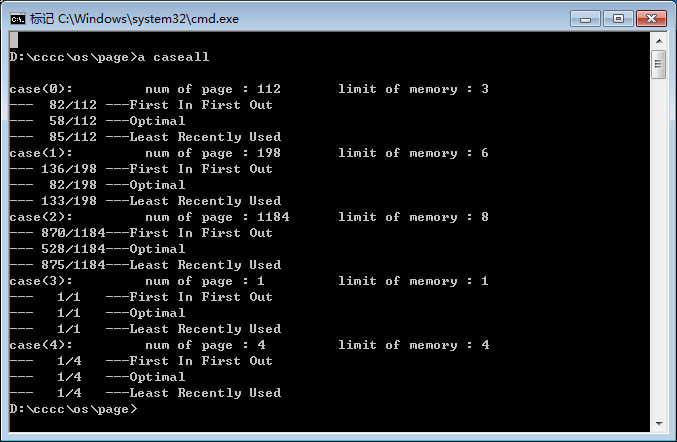
\includegraphics[scale = 0.7]{page.png}%%引用001.pdf首页
%\label{fig:screenshoot1}
%\end{figure}
%%%%%%%%%%%%%%%%%%%%%%%%%%%%%%%%%%%%%%%%%%%%%%%%%%%%%%%%
%\begin(figure)[ht]
%\centering
%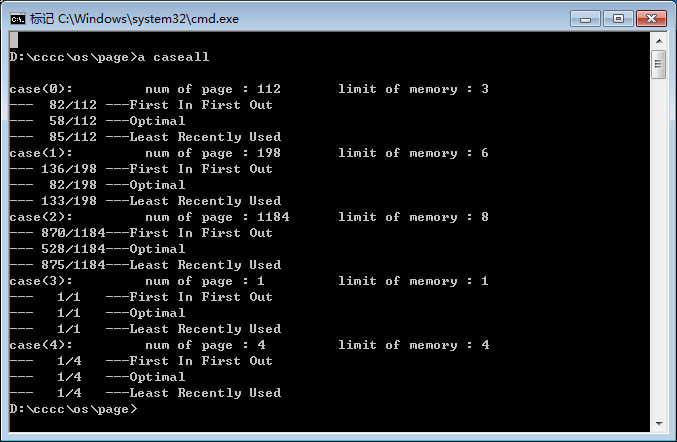
\includegraphics[scale = 0.5]{page.png}%%引用001.pdf首页
%\label{fig:screenshoot1}
%\end{figure}
\newpage
\section{详细代码}

%\begin{lstlisting}[language = C]
\begin{verbatim}
#include<stdio.h>
#include<stdlib.h>
int next = 0;
int rear = 0;
unsigned int swappage1(int flag,unsigned int page[],unsigned int mem[],
unsigned int start,unsigned int current,unsigned int max_memory,unsigned int num_of_page)
{
    if(!flag)return 0;
    int pos = next;
    next = (next + 1) % max_memory;
    return pos;
}
unsigned int swappage2(int flag,unsigned int page[],unsigned int mem[],
unsigned int start,unsigned int current,unsigned int max_memory,unsigned int num_of_page)
{
    unsigned int pos = 0;
    int maxv = -1;
    int i,j;
    if(!flag)return 0;
    for(i = 0; i < max_memory; i++)
    {
        int findflag = 0;
        for(j = start;j < num_of_page; j++)
        {
            if(page[j] == mem[i])
            {
                findflag = 1;
                if(j > maxv)
                {
                    maxv = j;
                    pos = i;
                }
                break;
            }
        }
        if(findflag)
        continue;
    /// if mem[i] end of page
    maxv = num_of_page;
    pos = i;
    return pos;
    }
    return pos;
}
unsigned int swappage3(int flag,unsigned int page[],unsigned int mem[],
unsigned int start,unsigned int current,unsigned int max_memory,unsigned int num_of_page)
{
    int pos = rear;
    /// in the queue
    int i;
    if(!flag)
    {
        int temp = mem[current];
        for(i = current; i != rear; i= (i - 1 + max_memory) % max_memory)
        {
            mem[i] = mem[(i - 1 + max_memory) % max_memory];
        }
        mem[rear] = temp;
        rear = (rear + 1) % max_memory;
        return pos;
    }
    else
    {
    /// not in queue
        rear = (rear + 1) % max_memory;
    return pos;
    }
}
int mainfun(unsigned int max_memory,unsigned int num_of_page,unsigned int mem[],
unsigned int page[],unsigned int (*swap)(int flag,unsigned int page[],unsigned int mem[],
unsigned int start,unsigned int current,unsigned int max_memory,unsigned int num_of_page))
{
    unsigned int i;
    unsigned int success = 0;
    unsigned int failed = 0;
    for (i = 0; i < max_memory; i++)
    {
        mem[i] = -1;
    }
    for (i = 0; i < num_of_page; i++)
    {
        int j;
        int flag = 0;
        for(j = 0;j < max_memory; j++)
        {
            /// if data in mem
            if(page[i] == mem[j])
            {
                flag = 1;
                break;
            }
        }
        /// if data in mem
        if(flag)
        {
            success++;
            swap(0,page,mem,i,j,max_memory,num_of_page);
            continue;
        }
        /// if data out mem
        /// still test
        int pos = swap(1,page,mem,i,j,max_memory,num_of_page);
        mem[pos] = page[i];
        failed++;
        continue;
    }
    /// compute failed rate
    printf("\n---%4u/%-4u", failed, failed + success);
    return 0;
}
int main1(int argc,char** argv,FILE *fp)
{
    int i;
    unsigned int max_memory;
    unsigned int num_of_page;
    fscanf(fp, "%u", &num_of_page);
    fscanf(fp, "%u", &max_memory);    
    unsigned int page[num_of_page];    
    unsigned int mem[max_memory];
    printf("\t num of page : %u\t limit of memory : %u", num_of_page, max_memory);
    for (i = 0; i < num_of_page; i++)
    {
        fscanf(fp, "%u",&page[i]);
    }
    /////////////////////////////
    /////////////////////////////
    mainfun(max_memory,num_of_page,mem,page,swappage1);printf("---First In First Out");
    mainfun(max_memory,num_of_page,mem,page,swappage2);printf("---Optimal");
    mainfun(max_memory,num_of_page,mem,page,swappage3);printf("---Least Recently Used");
    return 0;
}
int main(int argc,char** argv)
{
    int num_of_case;
    int i;
    FILE *fp;
    if (2 != argc)
    {printf("\nTips: a.exe data.txt");return 1;}
    fp = fopen(argv[1], "rt");
    if(NULL==fp){printf("\nFile Not Found");return 1;}
    fscanf(fp, "%u", &num_of_case);
    for(i = 0; i < num_of_case; i++)
    {
        printf("\ncase(%d):",i);
        main1(argc,argv,fp);
    }
    fclose(fp);
    return 0;
}
\end{verbatim}
%\end{lstlisting}
\end{document}